\section{Đề ôn thi giữa kỳ 2 toán 10}
\subsection{Phần trắc nghiệm}
Câu trắc nghiệm nhiều phương án lựa chọn. Học sinh trả lời từ
câu 1 đến câu 12. Mỗi câu hỏi học sinh \textit{chỉ chọn một} phương án.

\Opensolutionfile{ans}[Ans/Dapan]

\hienthiloigiaiex

%%%% Câu 1
\begin{ex}%[0D3H2-3]%[Dự án đề kiểm tra Toán khối 10 GHKII NH23-24-Dot 2- Thành Đức Trung]%[Đề số 5 - CTST]
\immini
{
Cho hàm số $y=f(x)=ax^2+bx+c$ có đồ thị như hình bên. Dấu của hệ số $a$ và biệt thức $\Delta$ là
\choice
{\True $a>0$, $\Delta>0$}
{$a<0$, $\Delta>0$}
{$a>0$, $\Delta=0$}
{$a<0$, $\Delta=0$}
}
{
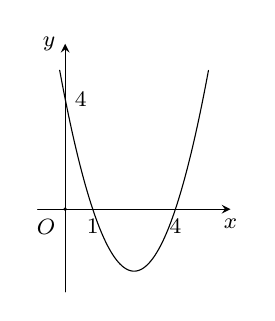
\begin{tikzpicture}[scale=0.7, font=\footnotesize, line join=round, line cap=round, >=stealth, xscale=0.5, yscale=0.5]
\draw[->](-1,0)--(6,0)node[below]{$x$};
\draw[->](0,-3)--(0,6)node[left]{$y$};
\draw[smooth, samples=100, domain=-0.2:5.2]plot(\x,{(\x)^2-5*(\x)+4});
;
\path
(0,0)node[below left]{$O$}
(1,0)node[below]{$1$}
(4,0)node[below]{$4$}
(0,4)node[right]{$4$}
;
\fill
(0,0)circle(2pt)
;
\end{tikzpicture}
}
\loigiai
{
Dựa vào đồ thị ta thấy, đồ thị hàm số cắt trục hoành tại hai điểm phân biệt và có bề lõm hướng lên trên nên $a>0$, $\Delta>0$.
}
\end{ex}

%%%% Câu 2
\begin{ex}%[0D7H2-1]%[Dự án đề kiểm tra Toán khối 10 GHKII NH23-24-Dot 2- Thành Đức Trung]%[Đề số 5 - CTST]
Bất phương trình nào sau đây có tập nghiệm là $S=\mathbb{R}\setminus\{2\}$.
\choice
{$x^2+4x+5\leq0$}
{$-2x^2+5x-11>0$}
{\True $-3x^2+12x-12<0$}
{$-3x^2+12x-12\geq0$}
\loigiai
{
Ta có
$$\begin{aligned}
& \ -3x^2+12x-12<0 \Leftrightarrow -3\left(x^2-4x+4\right)<0 \\
\Leftrightarrow & \ x^2-4x+4>0\Leftrightarrow \left(x-2\right)^2>0 \Leftrightarrow x\neq2.
\end{aligned}$$
Vậy bất phương trình $-3x^2+12x-12<0$ có tập nghiệm là $S=\mathbb{R}\setminus\{2\}$
}
\end{ex}

%%%% Câu 3
\begin{ex}%[0D7H1-2]%[Dự án đề kiểm tra Toán khối 10 GHKII NH23-24-Dot 2- Thành Đức Trung]%[Đề số 5 - CTST]
Cho tam thức bậc hai $f(x)=-x^2+5x-6$. Khi đó $f(x)>0$ khi và chỉ khi
\choice
{$x\in(-\infty;2)$}
{$x\in(3;+\infty)$}
{$x\in(2;+\infty)$}
{\True$x\in(2;3)$}
\loigiai
{
Ta có $-x^2+5x-6>0\Leftrightarrow 2<x<3$. Suy ra $x\in(2;3)$.
}
\end{ex}

%%%% Câu 4
\begin{ex}%[0D7H1-2]%[Dự án đề kiểm tra Toán khối 10 GHKII NH23-24-Dot 2- Thành Đức Trung]%[Đề số 5 - CTST]
Bảng xét dấu nào sau đây là của tam thức $f(x)=-x^2+4x-4$?
\choice
{

\begin{tikzpicture}[scale=1]
\tkzTabInit[nocadre=false, lgt=1.2, espcl=2.5, deltacl=0.6]{$x$/0.6, $f(x)$/0.6}{$-\infty$, $2$, $+\infty$}
\tkzTabLine{,+,0,-,}
\end{tikzpicture}
}
{

\begin{tikzpicture}[scale=1]
\tkzTabInit[nocadre=false, lgt=1.2, espcl=2.5, deltacl=0.6]{$x$/0.6, $f(x)$/0.6}{$-\infty$, $2$, $+\infty$}
\tkzTabLine{,-,0,+,}
\end{tikzpicture}
}
{\True 

\begin{tikzpicture}[scale=1]
\tkzTabInit[nocadre=false, lgt=1.2, espcl=2.5, deltacl=0.6]{$x$/0.6, $f(x)$/0.6}{$-\infty$, $2$, $+\infty$}
\tkzTabLine{,-,0,-,}
\end{tikzpicture}
}
{

\begin{tikzpicture}[scale=1]
\tkzTabInit[nocadre=false, lgt=1.2, espcl=2.5, deltacl=0.6]{$x$/0.6, $f(x)$/0.6}{$-\infty$, $2$, $+\infty$}
\tkzTabLine{,+,0,+,}
\end{tikzpicture}
}
\loigiai
{
Ta có $-\dfrac{b}{2a}=-\dfrac{4}{-2}=2$.\\
Mặt khác $a<0$ nên ta có bảng xét dấu
\begin{center}

\begin{tikzpicture}[scale=1]
\tkzTabInit[nocadre=false, lgt=1.2, espcl=2.5, deltacl=0.6]{$x$/0.6, $f(x)$/0.6}{$-\infty$, $2$, $+\infty$}
\tkzTabLine{,-,0,-,}
\end{tikzpicture}
\end{center}
}
\end{ex}

%%%% Câu 5
\begin{ex}%[0D7H3-1]%[Dự án đề kiểm tra Toán khối 10 GHKII NH23-24-Dot 2- Thành Đức Trung]%[Đề số 5 - CTST]
Tập nghiệm của phương trình $x-\sqrt{x-3}=\sqrt{3-x}+3$ là
\choice
{$S=\varnothing$}
{\True $S=\{3\}$}
{$S=[3;+\infty)$}
{$S=\mathbb{R}$}
\loigiai
{
Tập xác định $\mathscr{D}=\{3\}$.\\
Thay $x=3$ vào phương trình ta được $3=3$ (luôn đúng).\\
Suy ra $x=3$ là nghiệm của phương trình đã cho.\\
Vậy $S=\{3\}$.
}
\end{ex}

%%%% Câu 6
\begin{ex}%[0D7H3-1]%[Dự án đề kiểm tra Toán khối 10 GHKII NH23-24-Dot 2- Thành Đức Trung]%[Đề số 5 - CTST]
Phương trình $\sqrt{f(x)}=\sqrt{g(x)}$ tương đương với phương trình nào sau đây?
\choice
{$f(x)=g(x)$}
{$f^2(x)=g^2(x)$}
{$\hoac{ & f(x)\geq0\\ & f(x)=g(x)}$}
{\True$\heva{ & f(x)\geq0\\ & f(x)=g(x)}$}
\loigiai
{
Ta có $\sqrt{f(x)}=\sqrt{g(x)}\Leftrightarrow \heva{ & f(x)\geq0\\ & f(x)=g(x)}$.
}
\end{ex}

%%%% Câu 7
\begin{ex}%[0H5H1-3]%[Dự án đề kiểm tra Toán khối 10 GHKII NH23-24-Dot 2- Thành Đức Trung]%[Đề số 5 - CTST]
Trong mặt phẳng tọa độ $Oxy$, cho $\overrightarrow{a}=(-4;2)$; $\overrightarrow{b}=(2k;-k)$. Với giá trị nào của $k$ dưới đây thì $\overrightarrow{a}=\overrightarrow{b}$?
\choice
{$k=-\dfrac{1}{2}$}
{$k=2$}
{\True $k=-2$}
{Không tồn tại $k$}
\loigiai
{
Ta có $\overrightarrow{a}=\overrightarrow{b}\Leftrightarrow \heva{ & -4=2k\\ & 2=-k}\Leftrightarrow k=-2$.
}
\end{ex}

%%%% Câu 8
\begin{ex}%[0H5H3-2]%[Dự án đề kiểm tra Toán khối 10 GHKII NH23-24-Dot 2- Thành Đức Trung]%[Đề số 5 - CTST]
Trong mặt phẳng $Oxy$, cho $A(2;-3)$, $B(-4;1)$ và $C(-1;-1)$. Khẳng định nào dưới đây là đúng?
\choice
{\True $\overrightarrow{AB}=2\overrightarrow{AC}$}
{$\overrightarrow{AB}=\dfrac{1}{2}\overrightarrow{AC}$}
{$\overrightarrow{AB}=-2\overrightarrow{AC}$}
{$\overrightarrow{AB}=-\dfrac{1}{2}\overrightarrow{AC}$}
\loigiai
{
Ta có $\overrightarrow{AB}=(-6;4)$, $\overrightarrow{AC}=(-3;2)$. Suy ra $\overrightarrow{AB}=2\overrightarrow{AC}$.
}
\end{ex}

%%%% Câu 9
\begin{ex}%[0H9N3-2]%[Dự án đề kiểm tra Toán khối 10 GHKII NH23-24-Dot 2- Thành Đức Trung]%[Đề số 5 - CTST]
Phương trình tham số của đường thẳng $d$ đi qua $A(0;-2)$ và có véc-tơ chỉ phương $\overrightarrow{u}=(2;-3)$ là
\choice
{\True$\heva{ & x=2t\\ & y=-2-3t}$}
{$\heva{ & x=2\\ & y=-3-2t}$}
{$\heva{ & x=3t\\ & y=3+2t}$}
{$\heva{ & x=2+t\\ & y=-3-2t}$}
\loigiai
{
Phương trình tham số của đường thẳng $d$ đi qua $A(0;-2)$ và có véc-tơ chỉ phương $\overrightarrow{u}=(2;-3)$ là $\heva{ & x=2t\\ & y=-2-3t}$.
}
\end{ex}

%%%% Câu 10
\begin{ex}%[0H9N3-2]%[Dự án đề kiểm tra Toán khối 10 GHKII NH23-24-Dot 2- Thành Đức Trung]%[Đề số 5 - CTST]
Phương trình tham số của đường thẳng $d\colon \dfrac{x}{4}-\dfrac{y}{3}=1$ là
\choice
{$\heva{ & x=4+3t\\ & y=4t}$}
{$\heva{ & x=4-4t\\ & y=3t}$}
{\True$\heva{ & x=4+4t\\ & y=3t}$}
{$\heva{ & x=4-3t\\ & y=4t}$}
\loigiai
{
Ta có $\dfrac{x}{4}-\dfrac{y}{3}=1\Leftrightarrow 3x-4y-12=0$.\\
Một véc-tơ pháp tuyến của $d$ là $\overrightarrow{n}_{d}=(3;-4)$. Suy ra một véc-tơ chỉ phương của $d$ là $\overrightarrow{u}_{d}=(4;3)$.\\
Một điểm đường thẳng $d$ đi qua là $A(4;0)$.\\
Vậy phương trình tham số của $d$ là $\heva{ & x=4+4t\\ & y=3t.}$
}
\end{ex}

%%%% Câu 11
\begin{ex}%[0H9H4-2]%[Dự án đề kiểm tra Toán khối 10 GHKII NH23-24-Dot 2- Thành Đức Trung]%[Đề số 5 - CTST]
Phương trình đường tròn tâm $I(3;-2)$ và đi qua điểm $M(-1;1)$ là
\choice
{$(x+3)^2+(y-2)^2=5$}
{\True $(x-3)^2+(y+2)^2=25$}
{$(x-3)^2+(y+2)^2=5$}
{$(x-3)^2+(y-2)^2=25$}
\loigiai
{
Ta có $R=IM=5$.\\
Vậy phương trình đường tròn tâm $I(3;-2)$ và đi qua điểm $M(-1;1)$ là $(x-3)^2+(y+2)^2=25$.
}
\end{ex}

%%%% Câu 12
\begin{ex}%[0H9H4-2]%[Dự án đề kiểm tra Toán khối 10 GHKII NH23-24-Dot 2- Thành Đức Trung]%[Đề số 5 - CTST]
Phương trình đường tròn có đường kính $AB$ với $A(-1;2)$ và $B(3;2)$ là
\choice
{$(x+1)^2+(y+2)^2=4$}
{$(x+1)^2+(y-2)^2=16$}
{\True $(x-1)^2+(y-2)^2=4$}
{$(x-3)^2+(y-2)^2=16$}
\loigiai
{
Ta có $I(1;2)$, $R=2$.\\
Vậy phương trình đường tròn là $(x-1)^2+(y-2)^2=4$.
}
\end{ex}

\Closesolutionfile{ans}

\bangdapan{Dapan}

\subsection{Câu trắc nghiệm đúng sai}
Học sinh trả lời từ câu 1 đến câu 4.
Trong mỗi ý \circlenum{A}, \circlenum{B}, \circlenum{C} và \circlenum{D} ở mỗi câu, học sinh chọn đúng hoặc sai.
\setcounter{ex}{0}
\LGexTF
\Opensolutionfile{ansbook}[ansbook/DapanDS]
\Opensolutionfile{ans}[Ans/DapanT]
 %%%============EX_1==============%%%
 \begin{ex}%[0D7H1-4]%[Dự án đề kiểm tra Toán khối 10 GHKII NH23-24-Dot 2- Tô Ngọc Thy]%[Đề số 5 - CTST]
 	Cho biểu thức $f(x)=(3x-1)\left(3x^2-4x+1\right)$. Khi đó
 	\choiceTF
		  {$f(x)=0\Leftrightarrow\hoac{&x=-\frac{1}{3}\\&x=1}$}
		  {\True Với $x\in\left(-\infty;\dfrac{1}{3}\right)\cup\left(\dfrac{1}{3};1\right)$ thì $f(x)<0$}
		  {Với $x\in(1;+\infty)$ thì $f(x)<0$}
		  {\True Bảng xét dấu của biểu thức là
		  	\begin{center}
		  		\begin{tikzpicture}[scale=1, font=\footnotesize, line join=round, line cap=round, >=stealth]
		  		\tkzTabInit
		  		[lgt=3.5,espcl=1.5] % tùy chọn
		  		{$x$/.8,$3x-1$/.8,$3x^2-4x+1$/.8, $f(x)$/.8} % cột 1
		  		{$-\infty$,$\frac{1}{3}$,$1$,$+\infty$} % hàng 1 cột 2
		  		\tkzTabLine{, - ,0 , + , t , + }
		  		\tkzTabLine{, + ,t , - , $0$ , + }
		  		\tkzTabLine{, - ,$0$ , - , $0$ , +} 
		  		\end{tikzpicture}\end{center} } 
 	\loigiai{
 		Ta có $$f(x)=(3x-1)\left(3x^2-4x+1\right)=0\Leftrightarrow\hoac{&3x-1=0\\&3x^2-4x+1=0}\Leftrightarrow\hoac{&x=\frac{1}{3}\\&x=1.}$$
 		Bảng xét dấu
 		\begin{center}
 			\begin{tikzpicture}[scale=1, font=\footnotesize, line join=round, line cap=round, >=stealth]
 			\tkzTabInit
 			[lgt=3.5,espcl=1.5] % tùy chọn
 			{$x$/.8,$3x-1$/.8,$3x^2-4x+1$/.8, $f(x)$/.8} % cột 1
 			{$-\infty$,$\frac{1}{3}$,$1$,$+\infty$} % hàng 1 cột 2
 			\tkzTabLine{, - ,0 , + , t , + }
 			\tkzTabLine{, + ,t , - , $0$ , + }
 			\tkzTabLine{, - ,$0$ , - , $0$ , +} 
 			\end{tikzpicture}
 		\end{center}
 		Từ bảng xét dấu, $x\in\left(-\infty;\dfrac{1}{3}\right)\cup\left(\dfrac{1}{3};1\right)$ thì $f(x)<0$.
 	}
\end{ex}
 %%%============EX_2==============%%%
\begin{ex}%[0D7H2-5]%[Dự án đề kiểm tra Toán khối 10 GHKII NH23-24-Dot 2- Tô Ngọc Thy]%[Đề số 5 - CTST]
 	Cho phương trình $\left(\sqrt{x^2+2x-3}-2x+2\right)^2+\left(2-\sqrt{x+3}\right)^2=0$ $(^*)$. Khi đó
 	\choiceTF
 	{Điều kiện $x\geq 3$}
 	{Phương trình $(^*)$ có $3$ nghiệm phân biệt}
 	{$x=\dfrac{7}{3}$ là nghiệm của phương trình $(^*)$}
 	{\True Nghiệm của phương trình $(^*)$ nhỏ hơn $2$} 
 	\loigiai{
 		Ta có 
 		$$\left(\sqrt{x^2+2x-3}-2x+2\right)^2+\left(2-\sqrt{x+3}\right)^2=0\Leftrightarrow\heva{&\sqrt{x^2+2x-3}-2x+2=0\\&2-\sqrt{x+3}=0.}$$
 		Phương trình $2-\sqrt{x+3}=0\Leftrightarrow\sqrt{x+3}=2$ có nghiệm $x=1$.\\
 		Ta có $\sqrt{x^2+2x-3}-2x+2=0\Leftrightarrow\sqrt{x^2+2x-3}=2x-2$. $(2)$\\
 		Bình phương hai vế phương trình $(2)$, ta có\\
 		$x^2+2x-3=4x^2-8x+4\Leftrightarrow\hoac{&x=1\\&x=\frac{7}{3}}$ (điều thỏa mãn $2x-2>0$).\\
 		Tuy nhiên chỉ có $x=1$ thỏa mãn phương trình $2-\sqrt{x+3}=0$.\\
 		Vậy tập nghiệm của phương trình ban đầu là $S=\left\lbrace1\right\rbrace$.
 	}
\end{ex}
  %%%============EX_3==============%%%
\begin{ex}%[0H9H3-3]%[Dự án đề kiểm tra Toán khối 10 GHKII NH23-24-Dot 2- Tô Ngọc Thy]%[Đề số 5 - CTST]
  	Cho tam giác $MNP$ có phương trình đường thẳng $MN$ là $2x+y+1=0$, phương trình đường cao $MK$ ($K\in NP$) là $x+y-1=0$, phương trình đường cao $NQ$ ($Q\in MP$) là $3-y+4=0$. Khi đó
  	\choiceTF
  	{\True Điểm $M$ có tọa độ là $(-2;3)$}
  	{\True Điểm $N$ có tọa độ là $(-1;1)$}
  	{Phương trình đường thẳng $NP$ là $2x+y-3=0$}
  	{Phương trình đường thẳng $MP$ là $2x+3y-5=0$} 
  	\loigiai{
  		Tọa độ của điểm $M$ là nghiệm của hệ phương trình $$\heva{&2x+y+1=0\\&x+y-1=0}\Leftrightarrow\heva{&x=-2\\&y=3.}$$
  		Suy ra điểm $M$ có tọa độ là $(-2;3)$.\\
  		Tọa độ của điểm $N$ là nghiệm của hệ phương trình $\heva{&2x+y+1=0\\&3x-y+4=0}\Leftrightarrow\heva{&x=-1\\&y=1.}$\\
  		Suy ra điểm $N$ có tọa độ là $(-1;1)$.\\
  		Các đường cao $MK$ và $NQ$ có vec-tơ pháp tuyến lần lượt là $\vec{n_1}=(1;1)$, $\vec{n_2}=(3;-1)$.\\
  		Do đó các đường thẳng $NP$, $MP$ lần lượt nhận $\vec{n_3}=(1;-1)$, $\vec{n_4}=(1;3)$ làm vec-tơ pháp tuyến.\\
  		Phương trình đường thẳng chứa cạnh $NP$ đi qua điểm $N(-1;1)$ và có vec-tơ pháp tuyến $\vec{n_3}=(1;-1)$ là $$1(x+1)-1(y-1)=0\Leftrightarrow x-y+2=0.$$
  		Phương trình đường thẳng chứa cạnh $MP$ đi qua điểm $M(-2;3)$ và có vec-tơ pháp tuyến $\vec{n_4}=(1;3)$ là $$1(x+2)+3(y-3)=0\Leftrightarrow x+3y-7=0.$$
  	}
\end{ex}
   %%%============EX_4==============%%%
\begin{ex}%[0H9H4-3]%[Dự án đề kiểm tra Toán khối 10 GHKII NH23-24-Dot 2- Tô Ngọc Thy]%[Đề số 5 - CTST]
 	Cho đường tròn $(C)$ có tâm $I(-1;2)$ và tiếp xúc với đường thẳng $\Delta\colon x-2y+7=0$. Khi đó
 	\choiceTF
 	{$\mathrm{d}(I,\Delta)=\dfrac{3}{\sqrt{5}}$}
 	{\True Đường kính của đường tròn có độ dài bằng $\dfrac{4}{\sqrt{5}}$}
 	{\True Phương trình đường tròn là $(x+1)^2+(y-2)^2=\dfrac{4}{5}$}
 	{Đường tròn $(C)$ tiếp xúc với đường thẳng $\Delta$ tại điểm có hoành độ lớn hơn $0$} 
 	\loigiai{
 		Đường tròn $(C)$ có tâm $I$ và tiếp xúc với đường thẳng $\Delta$ nên có bán kính $$R=\mathrm{d}(I,\Delta)=\dfrac{\left| -1-4+7\right|}{\sqrt{1+4}}=\dfrac{2}{\sqrt{5}}.$$
 		Vậy phương trình đường tròn $(C)$ là $(x+1)^2+(y-2)^2=\dfrac{4}{5}$.\\
 		Đường tròn tiếp xúc với đường thẳng $\Delta$ tại điểm có hoành độ nhỏ hơn $0$.
 	}
\end{ex}
\Closesolutionfile{ans}
\Closesolutionfile{ansbook}

\begin{center}
	\textbf{\textsf{BẢNG ĐÁP ÁN ĐÚNG SAI}}
\end{center}
\input{Ansbook/DapanDS}

\subsection{Phần tự luận}

\hienthiloigiaibt
%%%=============BT_1=============%%%
\begin{bt}%[1D6V4-6]%[Dự án đề kiểm tra Toán khối 11 GHKII NH23-24-Dot 1 - Nguyễn Thế Duy]%[Deso05-CTST]
	Số lượng vi khuẩn $V$ trong phòng thí nghiệm tính theo công thức $s(t) = s_0 \cdot 2^t$ trong đó $s_0$ là số lượng vi khuẩn $V$ lúc đầu, $s(t)$ là số lượng vi khuẩn có trong $t$ phút. Biết sau $3$ phút thì số lượng vi khuẩn $V$ là $625$ nghìn con. Hỏi sau $9$ phút thì số lượng vi khuẩn $V$ là bao nhiêu?
\loigiai{
	Vì sau $3$ phút số lượng vi khuẩn $V$ là $625$ nghìn con nên 
 \begin{align*}
     625000 = s_0 \cdot 2^3 \Rightarrow s_0 = \dfrac{625000}{2^3}.
 \end{align*}
 Số lượng vi khuẩn $V$ sau $9$ phút là 
 \begin{align*}
     s(9) = \dfrac{625000}{2^3} \cdot 2^9 = 625000 \cdot 2^6 = 4 \cdot 10^7 \text{ (con).}
 \end{align*}
	}
\end{bt}
\begin{bt}%[1D6H2-3]%[Dự án đề kiểm tra Toán khối 11 GHKII NH23-24-Dot 1 - Nguyễn Thế Duy]%[Deso05-CTST]
	Cho số thực $a$ thỏa mãn $0 < a \neq 1$. Tính giá trị của biểu thức
 \begin{align*}
     A = 2\log_{2}{12} + 3\log_{2}{5} - \log_{2}{15} - \log_{2}{150}.
 \end{align*}
\loigiai{
	Ta có $\begin{aligned}[t]
	    A &= 2\log_{2}{12} + 3\log_{2}{5} - \left(\log_{2}{15} + \log_{2}{150} \right)\\
     &= \log_{2}{12^2 \cdot 5^3} - \log_{2}{15 \cdot 150}\\
     &= \log_{2}{\dfrac{18000}{2250}} = \log_{2}{8} = 3.
	\end{aligned}$
	}
\end{bt} 
\begin{bt}%[1D6V3-2]%[Dự án đề kiểm tra Toán khối 11 GHKII NH23-24-Dot 1 - Nguyễn Thế Duy]%[Deso05-CTST]
Tìm tất cả các giá trị $m$ để hàm số $y = \ln{\left(x^2 - 2x - m + 1 \right)}$ có tập xác định là $\mathbb{R}$.	
\loigiai{
	Hàm số các định với mọi $x \in \mathbb{R}$ khi và chỉ khi $x^2 - 2x - m + 1 > 0, \forall x \in \mathbb{R}$.\\
 Suy ra $\left(x-1 \right)^2 > m, \forall x\in \mathbb{R} \Rightarrow m < 0$.
	}
\end{bt} 
\begin{bt}%[1D6V4-6]%[Dự án đề kiểm tra Toán khối 11 GHKII NH23-24-Dot 1 - Nguyễn Thế Duy]%[Deso05-CTST]
	Số lượng của một loài vi khuẩn trong phòng thí nghiệm được tính theo công thức $S(t) = A \cdot e^{rt}$, trong đó $A$ là số lượng vi khuẩn ban đầu, $S(t)$ là số lượng vi khuẩn có sau $t$ (phút), $r$ là tỉ lệ tăng trưởng $\left(r>0 \right)$, $t$ (tính theo phút) là thời gian tăng trưởng. Biết rằng số lượng vi khuẩn ban đầu có $500$ con và sau $6$ giờ có $2000$ con. Hỏi ít nhất bao nhiêu giờ, kể từ lúc bắt đầu, số lượng vi khuẩn đạt ít nhất $120000$ con?
\loigiai{
	Ta có, sau $6$ giờ số lượng vi khuẩn là $2000$ con, tức là \begin{align*}
     2000 = 500 \cdot e^{r \cdot 350}
     \Leftrightarrow e^{r \cdot 360} = 4 \Leftrightarrow r = \dfrac{\ln4}{360} ~\left(\text{do } e>1 \right).
	\end{align*}
 Số lượng vi khuẩn đạt ít nhất $120000$ con, nghĩa là 
 \begin{align*}
     500 \cdot e^{\tfrac{\ln{4}}{360} \cdot t} \geq 120000 & \Leftrightarrow e^{\tfrac{\ln{4}}{360} \cdot t} \geq 240\\
     &\Leftrightarrow \dfrac{\ln{4}}{360} \cdot t \geq \ln{240} \Leftrightarrow t \geq \dfrac{360 \cdot \ln{240}}{\ln{4}} \approx 1423{,}24 ~\left(\text{phút} \right).
 \end{align*}
 Vậy sau ít nhất $24$ giờ thì số lượng vi khuẩn đạt ít nhất $120000$ con.
	}
\end{bt} 
\begin{bt}%[1D7V3-3]%[Dự án đề kiểm tra Toán khối 11 GHKII NH23-24-Dot 1 - Nguyễn Thế Duy]%[Deso05-CTST]
	Một vật được phóng theo phương thẳng đứng lên trên từ mặt đất, biết độ cao $h$ của nó (tính bằng mét) sau $t$ giây được cho bởi phương trình $h(t) = 24{,}5 t - 4{,}9 t^2$. Tìm vận tốc của vật khi nó chạm đất.
\loigiai{
	Khi vật chạm đất thì $h = 0 \Leftrightarrow 24{,}5 t - 4{,}9t^2 = 0 \Rightarrow t = 5$.\\
 Ta có $v(t) = h'(t) = 24{,}5 - 9{,}8t$ nên tốc độ của vật tại thời điểm nó chạm đất $t = 5$ là \begin{align*}
     v(5) = \left| h'(5) \right| = \left|24{,}5 - 9{,}8 \cdot 5 \right| = 24{,}5 \left(m/s \right).
 \end{align*}
	}
\end{bt} 
\begin{bt}%[1D7V3-1]%[Dự án đề kiểm tra Toán khối 11 GHKII NH23-24-Dot 1 - Nguyễn Thế Duy]%[Deso05-CTST]
	Tính đạo hàm cấp hai của hàm số $f(x) = x\sin{x} - 3$.
\loigiai{
	Ta có $y' = f'(x) = \left(x\sin{x} - 3 \right)' = \sin{x} + x\cos{x}$.\\
 Vậy $y'' = f''(x) = \left( \right)' = 2\cos{x} - x\sin{x}$.
	}
\end{bt} 
